\subsection{``Hello World!''}
We first try writing a simple macro that prints ''Hello World!'' in the log window of ImageJ. For this, we use a text editor that comes with Fiji, called ``script editor''. 
It has some convenient features such as automatic coloring of macro functions {In programming world, we call this feature ``syntax highlighter''}. 

If you are not using Fiji and using native ImageJ, it's no problem as there is a simpler but perfectly working text editor. Macros we write in this textbook works exactly same in both editors. If you want to use the simple text editor for the following tutorial, its usage is explained after the explanation about Fiji edior (page \pageref{part:nativeeditor}).   

Let's open the ``script editor'' 
by \ijmenu{[File -> New -> Script]}. It should look like figure \ref{fig_ScriptEditor}.
There should be a blank text field where you write your macro. Since the editor allows you to write different scripting languages as well, you should first select the language you are going to use.  
From script editor's own menu, select \ijmenu{[Language -> IJ1 Macro]}. 

Then, write your first macro as shown below (see also figure \ref{fig_ScriptEditor}). \\
\begin{lstlisting}[numbers=none]
print("Hello World!");
\end{lstlisting}

Don't ignore quotation marks, parenthesis and the semi-colon! 
Syntax highlighter offers automatic coloring of ImageJ functions, because you selected the language "IJ macro" in above. It increases the readability of codes. 

\begin{figure}[hbtp]
\begin{center}
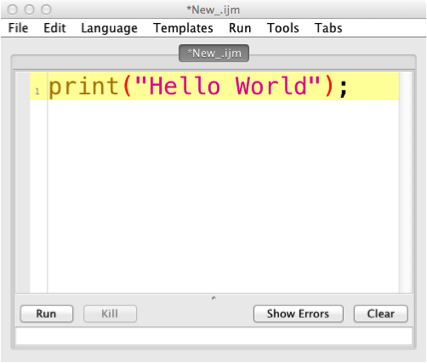
\includegraphics[scale=1.0]{fig/editor_helloworld_singleline.png}
\caption{Script Editor of the Fiji distribution} \label{fig_ScriptEditor}
\end{center}
\end{figure}

Then in the bottom-left corner of the script editor, there is a button labeled "Run". Clicking this, you will see that a log window is created (if it is already there, then it will have a new line) printing "Hello World!" (Figure \ref{fig_HelloWorldLog}). Another way to run the macro is via Script Editor menu,  \ijmenu{[Run -> Run]} . You could use Ctrl-R (Windows) or Command-R (OSX) as well.  

\begin{figure}[hbtp]
\begin{center}
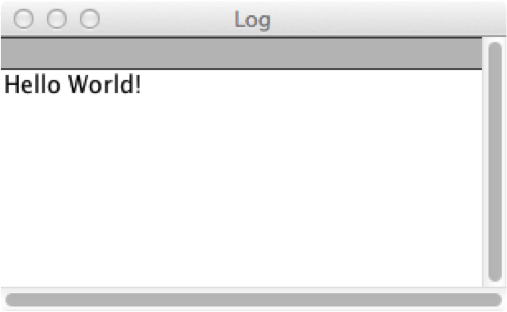
\includegraphics[scale=1.0]{fig/helloworld_logwindow.png}
\caption{Hello World Output} \label{fig_HelloWorldLog}
\end{center}
\end{figure}

Later when you want to start writing another macro, you could just create a new tab by \ijmenu{[File > New]} and then select \ijmenu{[Language -> ImageJ Macro]} again.

\subsubsection{Simple Text Editor in native ImageJ}
\label{part:nativeeditor}

If you are using native imageJ, the the macro editor launches by selecting \ijmenu{[PlugIns -> New -> Macro]} from the menu (\ref{fig_MacroEditor}). 
Please write the following line in the editor. 
\begin{lstlisting}[numbers=none]
print("Hello World!");
\end{lstlisting}
From the menu of the macro editor (in OSX, the menu switches to the editors own menu when the editor window is active), select [Macros > Run Macro]. You should then see "Hello World!" printed in the log window. 

The macro editor has simple debugger function, which is not present in Fiji script editor. Debugger assists you to correct mistakes in the code. ImageJ Macro can be written in any text editor such as "Notepad" in Windows but of course there is no debugger function available in this case.

\begin{figure}[htbp]
\begin{center}
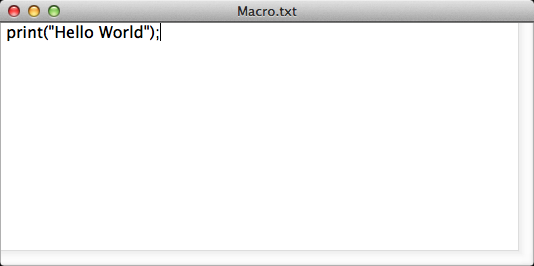
\includegraphics[scale=0.6]{fig/editor_helloworld_IJ_simple.png}
\caption{Macro Editor of ImageJ} \label{fig_MacroEditor}
\end{center}
\end{figure}


\subsubsection{Anatomy of ``Hello World!''}

Let's see more details of what the single line code we wrote is doing.

\ilcom{print()} is a build-in macro function that requests ImageJ to take the content within the parenthesis and print that out in the "Log" window. This content, which we genearlly call the \textit{argument} of the function, is an input value given to the function. The output of this function is the printed text in the Log window. Note that when a text is given as an argument, it must be surrounded by double quotes ("").
 
Where do we get information as such for other macro functions? The best reference for ImageJ macro functions is in the ImageJ web site
\footnote{\url{http://rsbweb.nih.gov/ij/developer/macro/functions.html}}. 
For example, you could find definition of \ilcom{print("")} function on the web site as quoted below:\\
%\item
\begin{indentCom}
%\begin{minipage}[c][18em][c]{0.85\textwidth}
\fbox{
\parbox[b][20em][c]{0.80\textwidth}{
\textbf{print(string)}\\
Outputs a string to the "Log" window. Numeric arguments are automatically converted to strings. 
The print() function accepts multiple arguments. For example, you can use print(x,y,width, height) 
instead of print(x+" "+y+" "+width+" "+height). 
If the first argument is a file handle returned by File.open(path), 
then the second is saved in the referred file (see SaveTextFileDemo).

Numeric expressions are automatically converted to strings using four decimal places, 
or use the \ilcom{d2s} function to specify the decimal places. 
For example, print(2/3) outputs "0.6667" but print(d2s(2/3,1)) outputs "0.7".

\dots
}
}
\end{indentCom}

As \ilcom{print} can do many things, its explanation is extraordinary long, but by carefully reading it, you will save time afterwards by the knowledge of wide spectrum of things that the \ilcom{print} function can do e.g. directly save text as a file. 

%If your machine is connected to the Internet, double clicking a function will automatically open the default web browser and guide you directly to the function help. From the menu the same could be done by \ijmenu{[Tools > Open Help for Macro Function]}.

Macro can be saved as a file.
In the editor, do \ijmenu{[File -> Save]}. Just save the file wherever you want in your file system. When you want to use the macro again, load the macro by \ijmenu{[File > Open]}.

%\begin{indentexercise}{1cm}
\begin{indentexercise}{1}
\item Add another line \texttt{"print("\textbackslash{}\textbackslash{}Clear");"} 
before the first line (below, code 1.51. don't forget the semi-colon at the end!). 
\item \lstinputlisting{code/code01_51.ijm}
Then test also another macro when you put the same line after "Hello World!". 
What happened? Any difference in the behavior? 
\item \lstinputlisting{code/code01_76.ijm}
\item \textbf{Answer}: The first code prints "Hello World!", while the second code prints nothing. This is becaise \ilcom{print("\textbackslash{}\textbackslash{}Clear")} is a command that clears the Log window. In the first code, ``Hello World'' is printed after the window clearing, and in the second case the Log window is wiped out right after the printing of ``Hello World''. Effectively it looks like nothing has happened.  
\end{indentexercise}

\begin{indentexercise}{2}
\item Try modifying the third line in code 1.51
and check that the modified text will be printed in the "Log" window. \\
\end{indentexercise}

\begin{indentexercise}{3}
\item Multiple macros can exist in a single file. We call this \textbf{"macro sets"}. To distinguish each macro, each they each should have a specific name. For this, each macro should start with a special word ``macro'' followed by the name of the macro, and then a pair of curly braces to encapsulate its macro functions. See the code below.  

\lstinputlisting{code/code01_8.ijm}

Modify the code you already wrote in the script editor to wrap it inside a pair of macro bounds, the curly braces (\ilcom{\{\}}).  Then copy and paste the same under the first macro. 
The second macro should be modified to have a different name. In the example shown in fig.
\ref{fig_MacroSetInMenu}, the second macro is named "print\_out2".
\begin{figure}[htbp]
\begin{center}
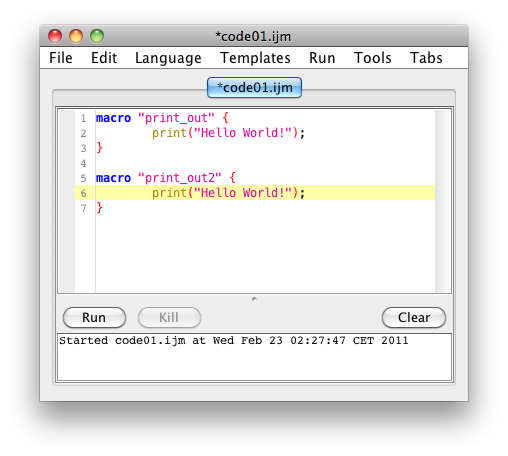
\includegraphics[scale=0.6]{fig/editor_MacroSet.png}
\caption{Macro Set} \label{fig_MacroSetInMenu}
\end{center}
\end{figure}
When macro is properly declared in this way, you could install the macro to have it as a menu item. To do so, in the editor menu select: 
\begin{indentFiji}
[Run -> Install Macro]).
\end{indentFiji}
In the main menu you should no be able to see the macro names under \ijmenu{[Plugins > Macros > ]}.

\begin{figure}[htbp]
\begin{center}
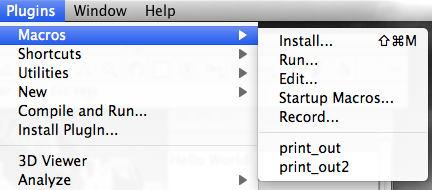
\includegraphics[scale=0.6]{fig/firstMacroSetInMenu.png}
\caption{Macro Now in ImageJ menu} \label{fig_MacroInMenu}
\end{center}
\end{figure}
\end{indentexercise}
